\section{初始化与精度}
\label{sec:nlipm-init-accuracy}

前两节都假设手里已经有一个能用的起点，也没有说算到什么程度可以停。本节要回答这两个问题：障碍路径和原始—对偶迭代分别需要怎样的起点，以及停下来的点能对原问题说什么。

\subsection{初始点的构造}
\label{sec:nlipm-initial-point}

两类方法对起点的要求不同。障碍法要计算$\log(-g_i(\bm{x}))$，所以每个迭代点都必须严格可行。原始—对偶方法的方程里不出现$\log(-g_i)$，它只要求$\bm{s},\bm{\lambda}>\bm{0}$，$\bm{x}$可以在可行域之外。

\paragraph{辅助可行性问题}
需要严格可行点时，可以先解一个以“最大违反量”为目标的问题：
\begin{equation}
 \min_{\bm{x},\rho}\ \rho\quad\text{s.t.}\quad g_i(\bm{x})\leq\rho\ (i=1,\ldots,m),\quad\bm{h}(\bm{x})=\bm{0}.
 \label{eq:nlipm-phase-one}
\end{equation}
这个问题的严格可行点是现成的：只要有一个满足等式的$\bm{x}$，取$\rho>\max_ig_i(\bm{x})$即可。线性等式可以解线性方程组得到这样的$\bm{x}$，非线性等式本身就是一个方程求根的问题，这里并没有绕过它。

设$\rho^\star$是最优值。在凸问题上，它的符号给出三种结论：

\begin{itemize}
 \item $\rho^\star<0$：最优点严格可行，可以作为障碍法的起点。
 \item $\rho^\star=0$：原问题可行或处在可行的边缘，但没有严格可行点。
 \item $\rho^\star>0$：原问题不可行。
\end{itemize}

在非凸问题上，算法只能找到局部解，$\rho>0$的局部解不能说明原问题不可行。

贯穿例从$\bm{x}^{(0)}=(2,1)^\top$开始，$\bm{g}=(3,-3)^\top$，取$\rho=4$就严格可行。解$\min\max\{x_1^2-x_2,\ x_2-4\}$时，$x_1=0$使第一项最小，再让$-x_2=x_2-4$，得到
\[
 \bm{x}=(0,2)^\top,\qquad\rho^\star=-2.
\]
这正是解析中心。图~\ref{fig:nlipm-phase-one}显示，随着$\rho$减小，放宽后的区域逐层收缩到这一点。实际上不必解到最优，一旦$\rho<0$就可以提前停下，这时得到的点已经是严格可行的。

\begin{BookInlineFigure}
  \centering
  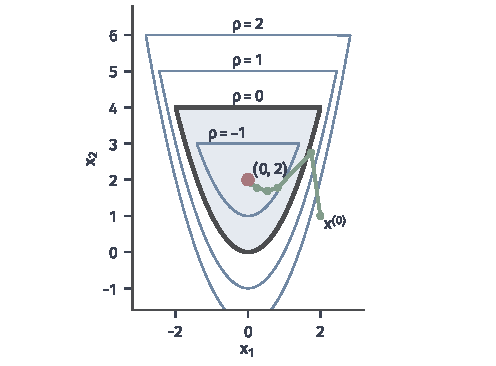
\includegraphics[width=84mm]{figures/05-optimization/06-constrained-optimization/matplotlib/nlipm-phase-one/figure.pdf}
  \caption{贯穿例的辅助问题~\eqref{eq:nlipm-phase-one}。蓝线是$\max_ig_i(\bm{x})=\rho$的水平集，深灰粗线是$\rho=0$，即原可行集的边界。绿线是从可行域外的$\bm{x}^{(0)}=(2,1)$出发、用障碍法解这个问题的迭代点，红点是解$(0,2)$，这里$\rho^\star=-2$。}
  \label{fig:nlipm-phase-one}
\end{BookInlineFigure}

\paragraph{从非零的原始残差开始}
原始—对偶方法不用先解辅助问题。任取$\bm{x}^{(0)}$，再选一个正的下限$\delta$，令
\begin{equation}
 s_i^{(0)}=\max\bigl\{-g_i(\bm{x}^{(0)}),\ \delta\bigr\},\qquad\lambda_i^{(0)}=\frac{\mu^{(0)}}{s_i^{(0)}}.
 \label{eq:nlipm-infeasible-start}
\end{equation}
这样所有乘积都等于$\mu^{(0)}$，起点在互补方程的意义下是居中的。约束已满足的分量，$\bm{r}_{\mathrm{p}}$是零，被违反的分量，$\bm{r}_{\mathrm{p}}$非零。

要记住的是，$\bm{s},\bm{\lambda}>\bm{0}$并不意味着$\bm{g}(\bm{x})+\bm{s}=\bm{0}$已经成立。正性是起点就满足的，松弛方程是迭代要逐步解的。在$\bm{r}_{\mathrm{p}}\neq\bm{0}$的点上，$s_i>0$也不告诉我们$g_i(\bm{x})<0$。

贯穿例取$\bm{x}^{(0)}=(2,1)^\top$，$\delta=1$，$\mu^{(0)}=1$，由式~\eqref{eq:nlipm-infeasible-start}得到
\[
 \bm{s}^{(0)}=\begin{bmatrix}1\\3\end{bmatrix},\qquad\bm{\lambda}^{(0)}=\begin{bmatrix}1\\1/3\end{bmatrix},\qquad\bm{r}_{\mathrm{p}}=\begin{bmatrix}4\\0\end{bmatrix}.
\]
仍取$\sigma=0.2$，按式~\eqref{eq:nlipm-condensed-data}算出
\[
 \tilde{\bm{H}}=\begin{bmatrix}19&-4\\-4&19/9\end{bmatrix},\qquad\bm{b}\approx\begin{bmatrix}-15.8\\3.133\end{bmatrix}.
\]
解出方向并回代，得到
\[
 \Delta\bm{x}\approx(-0.8636,\,-0.1521)^\top,\qquad\Delta\bm{s}\approx(-0.6977,\,0.1521)^\top.
\]

这一轮取到$\alpha=1$。线性规划中单位步会让等式残差归零，这里第一个分量却变成$\Delta x_1^2\approx0.7458$，这就是图~\ref{fig:nlipm-curved-residual}(b)的右端点。

第二轮$\alpha\approx0.946$，$r_{\mathrm{p},1}$降到$0.059$，再一轮之后降到$1.7\times10^{-5}$。图~\ref{fig:nlipm-infeasible-start}显示，残差下降虽然不再是精确的比例，但在这个例子上很快就跟上了互补量。

\begin{BookInlineFigure}
  \centering
  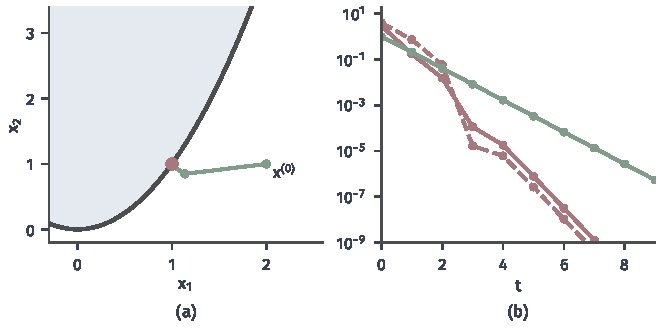
\includegraphics[width=112mm]{figures/05-optimization/06-constrained-optimization/matplotlib/nlipm-infeasible-start/figure.pdf}
  \caption{从可行域外启动，贯穿例，$\sigma=0.2$、$\eta=0.9$。(a)绿线是迭代点，从$(2,1)$进入可行域附近，红点是$\bm{x}^\star$。(b)红色虚线是$\lVert\bm{r}_{\mathrm{p}}\rVert_\infty$，红色实线是$\lVert\bm{r}_{\mathrm{d}}\rVert_\infty$，绿线是$\mu^{(t)}$。}
  \label{fig:nlipm-infeasible-start}
\end{BookInlineFigure}

\paragraph{不收敛到可行点的情形}
线性化的约束可能和当前的残差彼此矛盾。看不可行的一维约束$g(x)=x^2+1\leq0$。残差$x^2+1+s$在$s>0$上没有零点，迭代会被吸引到$x=0$、$s\to0$，这一点上$J=2x=0$，线性化的约束不再能改变残差。这是约束违反量的一个驻点，不是原问题的解。

对凸问题，这样的点可以变成证书。若存在$\bm{w}\geq\bm{0}$，使$\inf_{\bm{x}}\sum_iw_ig_i(\bm{x})>0$，则约束一定无解，因为可行点会让这个和不大于零。上面的例子取$w=1$，$\inf_x(x^2+1)=1>0$。非凸问题没有这样的结论，算法停在不可行驻点时，只能报告“这一带没有找到可行点”。

\paragraph{缺少严格可行点或约束退化}
内点法依赖的几个条件可能在模型层面就不成立，这时调参数没有用，要回到模型。图~\ref{fig:nlipm-no-interior}是三种常见情形。

图(a)的约束是两个相切的圆盘：
\[
 x_1^2+(x_2-1)^2\leq1,\qquad x_1^2+(x_2+1)^2\leq1.
\]
可行集只有原点，$\bm{C}^{\circ}$是空集。若目标是$\min x_1$，原点是唯一的可行点，但$\nabla f=(1,0)^\top$无法写成$(0,-2)^\top$和$(0,2)^\top$的组合，KKT条件不成立。这时根本没有路径。

图(b)是把一条等式拆成两条不等式，内部同样是空的。这种情形只需把等式约束显式写出来。

图(c)是重复的约束，例如把$g_1\leq0$写了两遍。这时$\bm{C}^{\circ}$不空，沿路径两个乘子相等，极限却不满足线性无关：在极限点，乘子的方向$(1,-1)$落在Newton矩阵的零空间里，矩阵奇异。算法的表现是$\bm{D}$很大的时候矩阵越来越病态，需要预处理去掉重复约束，或者加上$\delta_{\mathrm{c}}$。

\begin{BookInlineFigure}
  \centering
  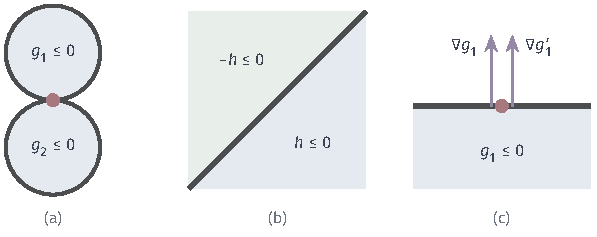
\includegraphics[width=101mm]{figures/05-optimization/06-constrained-optimization/tikz/nlipm-no-interior/figure.pdf}
  \caption{内点法的条件在模型层面失效的三种情形。(a)两个相切的圆盘（浅蓝），可行集只有红点，没有内部。(b)$h\leq0$和$-h\leq0$的公共部分是深灰的直线，同样没有内部。(c)同一条约束写了两遍，紫色箭头是两个相同的梯度，它们线性相关，乘子不唯一。}
  \label{fig:nlipm-no-interior}
\end{BookInlineFigure}

\subsection{停止条件}
\label{sec:nlipm-stopping}

迭代点永远在内部，算法只能在某处停下。这一小节回答什么量决定停止，以及停下的点能保证什么。

\paragraph{三项分别评价}
对参数$\mu$，定义误差
\begin{equation}
 E_\mu(\bm{z})=\max\Bigl\{\frac{\lVert\bm{r}_{\mathrm{d}}\rVert_\infty}{c_{\mathrm{d}}},\ \lVert\bm{r}_{\mathrm{e}}\rVert_\infty,\ \lVert\bm{r}_{\mathrm{p}}\rVert_\infty,\ \frac{\lVert\bm{S}\bm{\Lambda}\bm{1}-\mu\bm{1}\rVert_\infty}{c_{\mathrm{c}}}\Bigr\},
 \label{eq:nlipm-error}
\end{equation}
这里$c_{\mathrm{d}},c_{\mathrm{c}}\geq1$是按乘子大小确定的缩放，防止乘子很大时要求过严，贯穿例中都取$1$。$E_\mu$度量子问题的误差，$E_0$才度量原问题的KKT误差。最后的判据是$E_0\leq\varepsilon$。

\paragraph{参数小不等于解好了}
一个很小的$\mu$什么都说明不了，因为$\mu$是算法自己设定的数。起点取$\bm{\lambda}=10^{-3}\bm{1}$，$\mu$立刻就很小，而$\bm{r}_{\mathrm{d}}$的大小是$2$。反过来，$E_\mu$很小也只说明子问题解得好。

图~\ref{fig:nlipm-stop-staircase}是贯穿例上的一次运行，每当$E_\mu\leq0.1\mu$时，令$\mu\leftarrow0.2\mu$。第$6$轮$E_\mu\approx1.3\times10^{-5}$，子问题已经解得很准，而$E_0=0.04$，正好是当时的$\mu$。可以看到$E_0$紧贴$\mu$下降，$E_\mu$每次更新参数后跳起，再快速下降。

\begin{BookInlineFigure}
  \centering
  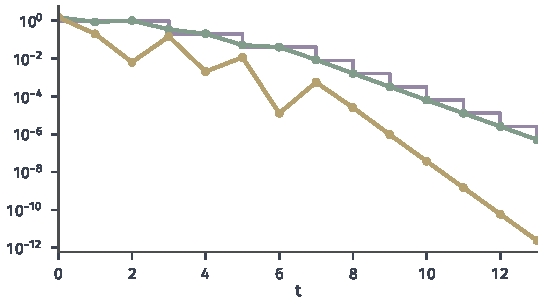
\includegraphics[width=92mm]{figures/05-optimization/06-constrained-optimization/matplotlib/nlipm-stop-staircase/figure.pdf}
  \caption{子问题误差与原问题误差，贯穿例，$\mu$只在$E_\mu\leq0.1\mu$时按$0.2$倍减小，对数纵轴。紫色折线是当前的$\mu$，绿线是原问题的KKT误差$E_0$，黄线是子问题误差$E_\mu$。$E_\mu$很小的时候，$E_0$仍然停在$\mu$的水平上。}
  \label{fig:nlipm-stop-staircase}
\end{BookInlineFigure}

\paragraph{内层精度与外层参数的配合}
由定义，$\lvert E_0-E_\mu\rvert\leq\mu/c_{\mathrm{c}}$，所以把$E_\mu$解得比$\mu$小很多并没有好处，$E_0$反正停在$\mu$的量级。常用的规则是：内层解到$E_\mu\leq\kappa\mu$，再更新参数
\begin{equation}
 \mu^+=\max\Bigl\{\frac{\varepsilon}{10},\ \min\bigl\{\tau\mu,\ \mu^{1+\theta}\bigr\}\Bigr\},
 \label{eq:nlipm-mu-update}
\end{equation}
其中$\kappa>0$，$\tau\in(0,1)$，$\theta\in(0,1)$。$\mu$大时线性减小，$\mu$小时超线性减小。下限$\varepsilon/10$防止参数比容差小太多，否则$\bm{D}$的数值徒然变大，矩阵更病态，而精度并不提高。

\paragraph{近似点能保证什么}
下面的定理说明残差小怎样转化成目标误差，它把定理~\ref{thm:nlipm-gap}推广到迭代点不在路径上、残差不为零的情形。

\begin{theorem}[近似点的目标误差]
\label{thm:nlipm-approx-certificate}
设$f$、$g_i$凸且可微，$\bm{h}(\bm{x})=\bm{A}\bm{x}-\bm{b}$，$(\bm{x},\bm{s},\bm{\lambda},\bm{\nu})$满足$\bm{\lambda}\geq\bm{0}$，残差如式~\eqref{eq:nlipm-residuals}定义。设$\bm{x}^\star$是最优解，$R\geq\lVert\bm{x}-\bm{x}^\star\rVert_2$。则
\begin{equation}
 f(\bm{x})-f^\star\leq\bm{\lambda}^\top\bm{s}-\bm{\lambda}^\top\bm{r}_{\mathrm{p}}-\bm{\nu}^\top\bm{r}_{\mathrm{e}}+\lVert\bm{r}_{\mathrm{d}}\rVert_2R.
 \label{eq:nlipm-approx-upper}
\end{equation}
若$(\bm{\lambda}^\star,\bm{\nu}^\star)$是一组KKT乘子，则还有
\begin{equation}
 f(\bm{x})-f^\star\geq-(\bm{\lambda}^\star)^\top\bm{g}(\bm{x})-(\bm{\nu}^\star)^\top\bm{r}_{\mathrm{e}}.
 \label{eq:nlipm-approx-lower}
\end{equation}
\end{theorem}

\begin{proof}
由$\bm{\lambda}\geq\bm{0}$和$\bm{x}^\star$可行，有
\[
 f^\star\geq\mathcal{L}(\bm{x}^\star,\bm{\lambda},\bm{\nu}).
\]
函数$\mathcal{L}(\cdot,\bm{\lambda},\bm{\nu})$是凸的，在$\bm{x}$处的梯度是$\bm{r}_{\mathrm{d}}$，于是
\[
 \mathcal{L}(\bm{x}^\star,\bm{\lambda},\bm{\nu})\geq\mathcal{L}(\bm{x},\bm{\lambda},\bm{\nu})+\bm{r}_{\mathrm{d}}^\top(\bm{x}^\star-\bm{x})\geq\mathcal{L}(\bm{x},\bm{\lambda},\bm{\nu})-\lVert\bm{r}_{\mathrm{d}}\rVert_2R.
\]
代入$\bm{g}(\bm{x})=\bm{r}_{\mathrm{p}}-\bm{s}$和$\bm{h}(\bm{x})=\bm{r}_{\mathrm{e}}$，$\mathcal{L}(\bm{x},\bm{\lambda},\bm{\nu})$展开为
\[
 f(\bm{x})-\bm{\lambda}^\top\bm{s}+\bm{\lambda}^\top\bm{r}_{\mathrm{p}}+\bm{\nu}^\top\bm{r}_{\mathrm{e}}.
\]
整理即得式~\eqref{eq:nlipm-approx-upper}。

对下界，$\bm{x}^\star$是凸函数$\mathcal{L}(\cdot,\bm{\lambda}^\star,\bm{\nu}^\star)$的最小点，并且由互补，这个最小值等于$f^\star$，于是
\[
 f^\star\leq\mathcal{L}(\bm{x},\bm{\lambda}^\star,\bm{\nu}^\star)=f(\bm{x})+(\bm{\lambda}^\star)^\top\bm{g}(\bm{x})+(\bm{\nu}^\star)^\top\bm{h}(\bm{x}).
\]
移项即得式~\eqref{eq:nlipm-approx-lower}。
\end{proof}

式~\eqref{eq:nlipm-approx-upper}右端的第一项是互补量，其余三项是残差被乘子和距离放大的部分。这正是第~\ref{chap:lp-interior-point}章不可行点上间隙公式的非线性版本。下界说明，点略微不可行时目标可以低于$f^\star$，低的幅度由违反量乘以最优乘子决定。

用表~\ref{tab:nlipm-run}中$t=4$的点核对。这时互补量和两个残差项是
\[
 \bm{\lambda}^\top\bm{s}\approx3.82\times10^{-3},\quad\lvert\bm{\lambda}^\top\bm{r}_{\mathrm{p}}\rvert\approx8.9\times10^{-6},\quad\lVert\bm{r}_{\mathrm{d}}\rVert_2\approx2.5\times10^{-5}.
\]
可行集的直径不超过$4.5$，取$R=4.5$，上界约为$3.92\times10^{-3}$。实际误差是$1.92\times10^{-3}$，确实在界内。

\paragraph{始终按原问题报告}
内点法的内部变量经过松弛、缩放，矩阵可能经过正则化，交付时都要回到原问题上算一遍。可行性按$\max_i\max\{g_i(\bm{x}),0\}$和$\lVert\bm{h}(\bm{x})\rVert_\infty$计算，而不是$\lVert\bm{r}_{\mathrm{p}}\rVert_\infty$，因为$s_i>0$时残差小并不排除$g_i(\bm{x})$略大于零。互补按$\lambda_i\lvert g_i(\bm{x})\rvert$计算，驻定按未缩放的梯度计算。

三种常见的修改都可能制造假象。矩阵正则化只改变方向，不改变残差的定义，所以它本身不影响判据，但$\delta_{\mathrm{c}}$较大时迭代可能停在一个并不满足等式的点上。把约束放宽成$g_i\leq\epsilon$的实现，要说明放宽量。恢复步骤之后乘子往往被重置，这时要用新的乘子重新计算$\bm{r}_{\mathrm{d}}$，不能沿用恢复之前的数值。

收敛到一个$E_0$很小的点，在非凸问题上也只说明这一点近似满足KKT条件。若需要二阶信息，还要看最后一次分解时是否用过$\delta_{\mathrm{w}}>0$，用过说明约化Hessian在该点并不正定。
